% Diagrama 1: flujo metodológico general
% Compila en Overleaf con pdfLaTeX o XeLaTeX.
\documentclass[border=12pt]{standalone}
\usepackage{iftex}
\ifPDFTeX
  \usepackage[utf8]{inputenc}
  \usepackage[T1]{fontenc}
  \usepackage[scaled]{helvet}
\else
  \usepackage{fontspec}
  \setsansfont{texgyreheros}[Extension=.otf, UprightFont=*-regular,
    BoldFont=*-bold, ItalicFont=*-italic, BoldItalicFont=*-bolditalic, Scale=0.95]
\fi
\renewcommand{\familydefault}{\sfdefault}
\usepackage{tikz}
\usetikzlibrary{arrows.meta, positioning}

\definecolor{azul}{HTML}{1F5A96}
\definecolor{verde}{HTML}{2E7D32}
\definecolor{morado}{HTML}{6A1B9A}
\definecolor{naranja}{HTML}{E07B00}
\definecolor{gris}{HTML}{455A64}

\begin{document}
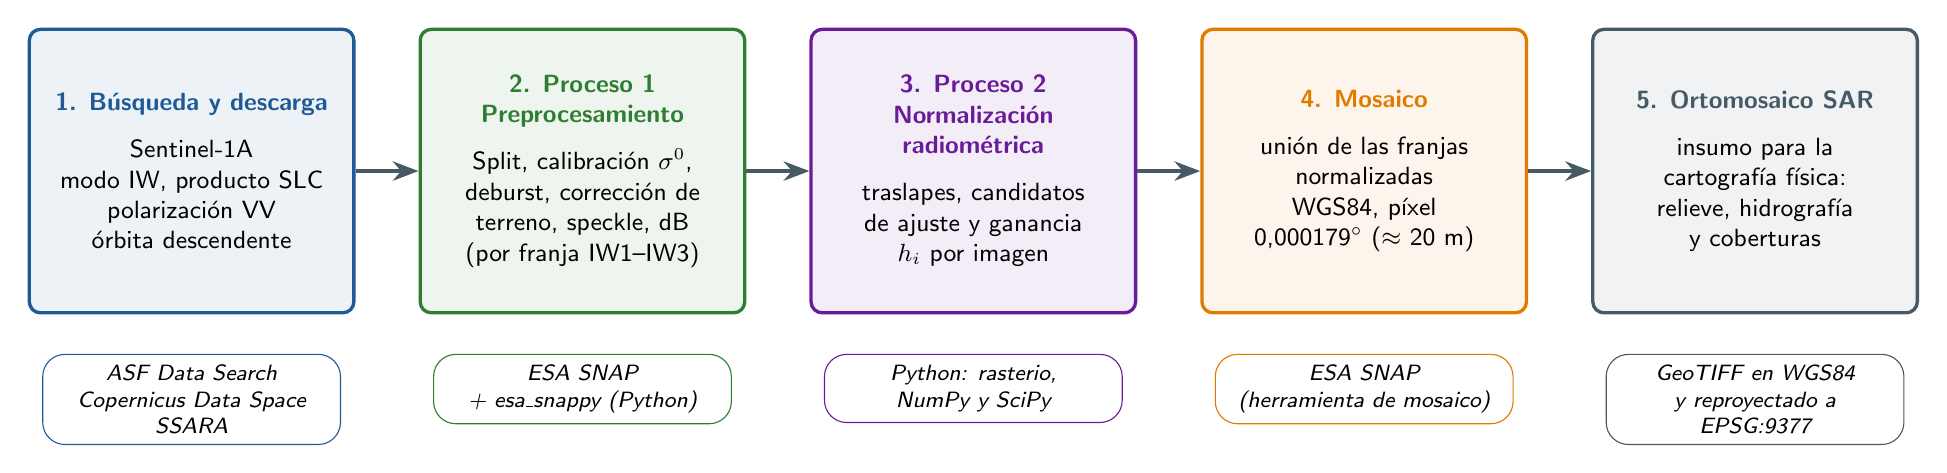
\begin{tikzpicture}[
  >=Stealth,
  fase/.style={rectangle, rounded corners=4pt, draw=#1, line width=1.2pt,
               fill=#1!8, text width=3.7cm, minimum height=3.6cm,
               align=flush center, font=\small, inner sep=6pt},
  herr/.style={rectangle, rounded corners=8pt, draw=#1, fill=white,
               text width=3.5cm, align=flush center, font=\footnotesize\itshape,
               inner sep=4pt},
  flecha/.style={->, line width=1.4pt, draw=gris}
]

\node[fase=azul] (f1) {\textbf{\color{azul}1. Búsqueda y descarga}\\[6pt]
  Sentinel-1A\\ modo IW, producto SLC\\ polarización VV\\ órbita descendente};
\node[fase=verde, right=8mm of f1] (f2) {\textbf{\color{verde}2. Proceso 1}\\
  \textbf{\color{verde}Preprocesamiento}\\[6pt]
  Split, calibración $\sigma^0$,\\ deburst, corrección de\\ terreno, speckle, dB\\ (por franja IW1--IW3)};
\node[fase=morado, right=8mm of f2] (f3) {\textbf{\color{morado}3. Proceso 2}\\
  \textbf{\color{morado}Normalización}\\
  \textbf{\color{morado}radiométrica}\\[6pt]
  traslapes, candidatos\\ de ajuste y ganancia\\ $h_i$ por imagen};
\node[fase=naranja, right=8mm of f3] (f4) {\textbf{\color{naranja}4. Mosaico}\\[6pt]
  unión de las franjas\\ normalizadas\\ WGS84, píxel\\ 0,000179$^\circ$ ($\approx$ 20 m)};
\node[fase=gris, right=8mm of f4] (f5) {\textbf{\color{gris}5. Ortomosaico SAR}\\[6pt]
  insumo para la\\ cartografía física:\\ relieve, hidrografía\\ y coberturas};

\foreach \a/\b in {f1/f2, f2/f3, f3/f4, f4/f5}
  \draw[flecha] (\a.east) -- (\b.west);

\node[herr=azul,    below=5mm of f1] {ASF Data Search\\ Copernicus Data Space\\ SSARA};
\node[herr=verde,   below=5mm of f2] {ESA SNAP\\ + esa\_snappy (Python)};
\node[herr=morado,  below=5mm of f3] {Python: rasterio,\\ NumPy y SciPy};
\node[herr=naranja, below=5mm of f4] {ESA SNAP\\ (herramienta de mosaico)};
\node[herr=gris,    below=5mm of f5] {GeoTIFF en WGS84\\ y reproyectado a\\ EPSG:9377};

\end{tikzpicture}
\end{document}
